\documentclass[conference]{IEEEtran}
\IEEEoverridecommandlockouts
% The preceding line is only needed to identify funding in the first footnote. If that is unneeded, please comment it out.
\usepackage{cite}
\usepackage{amsmath,amssymb,amsfonts}
\usepackage{algorithm}
\usepackage{algorithmic}
\usepackage{graphicx}
\usepackage{textcomp}
\usepackage{xcolor}
\usepackage{listings}                           %顯示code用的
\usepackage{fontspec}                           %設定字體
\usepackage[CheckSingle, CJKmath]{xeCJK}
\usepackage{CJKulem}
\usepackage{listings}
\usepackage{color} %red, green, blue, yellow, cyan, magenta, black, white
\usepackage{float}

\definecolor{mygreen}{RGB}{28,172,0} % color values Red, Green, Blue
\definecolor{mylilas}{RGB}{170,55,241}

% \setmainfont{Consolas}
%\setmonofont{Ubuntu Mono}
% \setmonofont{Consolas}
% \setCJKmainfont{Noto Sans CJK TC}
% \XeTeXlinebreaklocale "zh"                      %中文自動換行

\def\BibTeX{{\rm B\kern-.05em{\sc i\kern-.025em b}\kern-.08em
    T\kern-.1667em\lower.7ex\hbox{E}\kern-.125emX}}

\begin{document}
\title{Firefly Algorithm with Different Methods for Multilevel Image Thresholding Selection\\
% {\footnotesize \textsuperscript{*}Note: Sub-titles are not captured in Xplore and should not be used}
% \thanks{Identify applicable funding agency here. If none, delete this.}
}

\author{\IEEEauthorblockN{1\textsuperscript{st} Zih Jie Lin}
\IEEEauthorblockA{\textit{Computer Science Information Engineering.} \\
\textit{Fu Jen Catholoic University}\\
New Taipei City, Taiwan \\
406261597@gapp.fju.edu.tw}
}
% \and
% \IEEEauthorblockN{2\textsuperscript{nd} Given Name Surname}
% \IEEEauthorblockA{\textit{dept. name of organization (of Aff.)} \\
% \textit{name of organization (of Aff.)}\\
% City, Country \\
% email address or ORCID}
% \and
% \IEEEauthorblockN{3\textsuperscript{rd} Given Name Surname}
% \IEEEauthorblockA{\textit{dept. name of organization (of Aff.)} \\
% \textit{name of organization (of Aff.)}\\
% City, Country \\
% email address or ORCID}
% \and
% \IEEEauthorblockN{4\textsuperscript{th} Given Name Surname}
% \IEEEauthorblockA{\textit{dept. name of organization (of Aff.)} \\
% \textit{name of organization (of Aff.)}\\
% City, Country \\
% email address or ORCID}
% \and
% \IEEEauthorblockN{5\textsuperscript{th} Given Name Surname}
% \IEEEauthorblockA{\textit{dept. name of organization (of Aff.)} \\
% \textit{name of organization (of Aff.)}\\
% City, Country \\
% email address or ORCID}
% \and
% \IEEEauthorblockN{6\textsuperscript{th} Given Name Surname}
% \IEEEauthorblockA{\textit{dept. name of organization (of Aff.)} \\
% \textit{name of organization (of Aff.)}\\
% City, Country \\
% email address or ORCID}

\maketitle

% \begin{abstract}
% \end{abstract}

% \begin{IEEEkeywords}
% \end{IEEEkeywords}

\begin{abstract}
Image Thresholding is one of common technique in digitail image processing. The main probelem is how to select the threshold. To solve the problem, this paper apply the algorithm in \cite{b1}, a MET algorithm base on the firefly algorithm. Then revise the algorithm in initialize part. Finally, evaluate the performance between two revise algorithm.
\end{abstract}

\begin{IEEEkeywords}
multilevel thresholding, firefly algorithm, particle warm optimizationl, maximum entropy
\end{IEEEkeywords}

\section{Introduction}
Thresholding is the simple way to segment images. It need to thresholds for bi-level thresholding or multilevel thresholding to implment image segmentation. Bi-level thresholding chooses one threshold and the pixels in image will be divide into two class. Multilevel thresholding selects $N$ threshold and the pixels in image will be divide into $N+1$ group.

Image thresholding can be divide into two class, parametric and nonparametric. Parametric approaches use the distibution of graylevel to determine thresholding. Nonparametric thresholding approaches use some criteria, like entropy and variance, to obtain thresholds. For example, Otsu's algorithm, a well-known algorithm, obtains thresholds by maximizing the between-class variance.

Particle swarm optimization, propose in 1995, use particles to imitate social animals, like human and insects. Every particle has own position and velocity. The algorithm remeber the best of each particle ($p_{best}$) and the best of all particles ($g_{best}$). Every epoch, the velocity of each particle will change base on $p_{best}$ and $g_{best}$.

In this paper, an algorithm, maximum entropy based firefly thresholding (MEFFT) algorithm, in \cite{b1} first applied here. The algorithm is based on firefly algorithm. Firefly algorithm is one kind of particle swarm optimization. The algorithm use maximum entropy as criterion functions. This paper then modify the initialization part. The detail will be discaussed in Section 2. Experiment will shown in Section 3. Finally, conclusion will be in Section 4.

\section{Related work}
\subsection{Maximum entropy thresholding algorithm}
Maximum entropy thresholding algorithm, which first propose in \cite{b3}, was originally used for bi-level thresholding. It also can be applied in multilevel thresholding. THe problem is described as below:
\begin{itemize}
    \item There are $L$ gray levels in a given image $I$, the the gray level are in [0,L-1].
    \item $h(i)$ denotes the number of pixels with gray level $i$.
    \item $N$ denotes the total number pixels in image $I$.
    \item $P(i)=H(i)/N$, $P(i)$ means the proportion of the gray level $i$ in image $I$.
    \item $t_1,t_2,t_3,...,t_D$ is the selected threshold in given image $I$.
\end{itemize}
Based on above defintion, a objective function $\phi$ is defined. Its goal is to maximize: $\phi([t_1,t_2,t_3,...,t_D])=H_0+H_1+H_2+...+H_D$, where

\begin{equation}
\begin{aligned}
    \label{movement}
    H_0=-\sum\limits_{i=0}^{t_1-1}\frac{P_i}{\omega_0}ln\frac{P_i}{\omega_0},\omega_0=\sum\limits_{i=0}^{t_1-1}P_i\\
    H_1=-\sum\limits_{i=t_1}^{t_2-1}\frac{P_i}{\omega_0}ln\frac{P_i}{\omega_0},\omega_0=\sum\limits_{i=t_1}^{t_2-1}P_i\\
    ...\\
    H_D=-\sum\limits_{i=t_D}^{L-1}\frac{P_i}{\omega_0}ln\frac{P_i}{\omega_0},\omega_0=\sum\limits_{i=t_D}^{L-1}P_i
\end{aligned}
\end{equation}

When generating solutions in maximum entropy based firefly thresholding algorithm, objective function $\phi$ is used as fitness function to evaluate solutions.

\subsection{Firefly algorithm}
Firefly algorithm was proposed by Xin-she Yang \cite{b4} in 2008. In that paper, there are three idealized rules:
\begin{itemize}
    \item All fireflies are unisex so that one firefly will be attracted to other fireflies regardless of their sex.
    \item Attractiveness is proportional to their brightness, thus for any two flashing fireflies, the less brighter one will move towards the brighter one. If there is no brighter than a particular firefly, it will move randomly.
    \item The brightness of a firefly is affected or determined by the landscape of the fitness function $\phi$.
\end{itemize}

The fireflies' attractiveness is inversely proportional to the distance between them. For any two fireflies, namely firefly $i$ and firefly $j$, the distance $r_{i,j}$ is:

\begin{equation}
    \label{distance}
    r_{i,j}=||x_i-x_j||=\sqrt{\sum\limits_{k=i}^{c}(x_{i,k}-x_{j,k})^2}
\end{equation}

And the brightness between them is:

\begin{equation}
    \label{brightness}
    \beta\leftarrow\beta_0 e^{-\gamma r_{i,j}}
\end{equation}

where $\beta_0$ is the attractiveness at $r_{i,j}=0$, $\gamma$ is the light absorption coefficient at the source. Both them are hyperparameter. 

The movement of the firefly $i$ to another firefly $j$, whose brightness is higher than firefly $i$, is:

\begin{equation}
\begin{aligned}
    \label{movement}
    x_{i,k}=\leftarrow (1-\beta)x_{i,k}+\beta x_{j,k}+u_{i,k}\\
    u_{i,k}=\alpha(U(0,1)-\frac{1}{2})
\end{aligned}
\end{equation}

Where $U(0,1)$ are random number generated from uniform distibution from $0$ to $1$.

After movement for all fireflies. The best firefly will be randomly move:

\begin{equation}
\begin{aligned}
    \label{best firefly movement}
    x_{i^{max},k}=x_{i^{max},k}+u_{i^{max},k}
    u_{i^{max},k}=\alpha(U(0,1)-\frac{1}{2})
\end{aligned}
\end{equation}

\begin{algorithm}
\begin{algorithmic}[1]
    \STATE $\phi$, the fitness function to evaluate solutions.
    \STATE Parameters: $m, D,\beta_0,\alpha,\gamma,ML$ (the maximum iteration number) 
    \STATE $x=[x_1,x_2,...,x_m],$ the fireflies solutions.
    \STATE $x_i=[x_{i,1},x_{i,2},...,x_{i,D}],$ any D-dimensional firefly solution.
    \STATE initialize x
    \FOR{$ml\gets 1,ML$}
        \STATE $i^{max}=max_{i}\phi(x_i)$
        \FOR{$i\gets 1, m$}
            \FOR{$j\gets 1, m$}
                \IF {$\phi(x_i)<\phi(x_j)$}
                    \STATE $r_{i,j}=||x_i-x_j||=\sqrt{\sum\limits_{k=i}^{c}(x_{i,k}-x_{j,k})^2}$
                    \STATE $\beta\leftarrow\beta_0 e^{-\gamma r_{i,j}}$
                    \FOR{$k\gets 1, D$}
                        \STATE $u_{i,k}=\alpha(U(0,1)-\frac{1}{2})$
                        \STATE $x_{i,k}=\leftarrow (1-\beta)x_{i,k}+\beta x_{j,k}+u_{i,k}$
                    \ENDFOR
                \ENDIF
            \ENDFOR
        \ENDFOR
        \FOR{$k\gets 1, D$}
            \STATE $u_{i^{max},k}=\alpha(U(0,1)-\frac{1}{2})$
            \STATE $x_{i^{max},k}=x_{i^{max},k}+u_{i^{max},k}$
        \ENDFOR
    \ENDFOR
\end{algorithmic}
\caption{The detail of algorithm}
\end{algorithm}

\subsection{Initialize fireflies}
In the algorithm in \cite{b1}, the initialization of the firefly just set a constant value. This paper will use two different methods. Fiset method(method 1) is generating all fireflies in random in $[0,L-1]$. Second method(method 2) is dividing gray level into $D$ parts. For $i^{th}$ soution of each firefly, generating in $[\frac{L-1}{D}*(i-1),\frac{L-1}{D}*(i)]$, where $i\in[1,D]$ and $D$ is the number of thresholds. 

The paper will compare this two methods in the next section.

\section{Experiment}

The experiment are running on python 3.7.2. The parameters described below. All of the parameters are smae as \cite{b1}.
\begin{itemize}
    \item $\alpha$: 0.01
    \item $\beta_0$: 1
    \item $\gamma$: 1.0
    \item Size of firefly: 50
    \item Number of iteration: 100
\end{itemize}

This paper use 11 images in experiment. The images are shown below.

\begin{figure}[H]
    \centerline{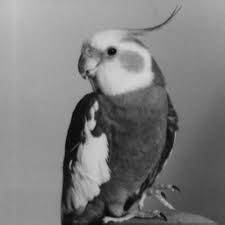
\includegraphics[width=3cm]{picture/bird.png}}
    \caption{bird}
    \label{bird}
\end{figure}

\begin{figure}[H]
    \centerline{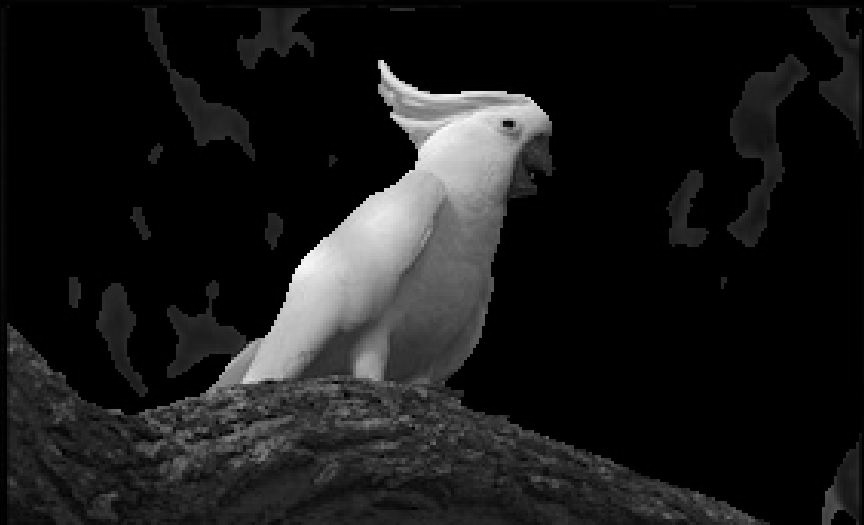
\includegraphics[width=3cm]{picture/bird2.png}}
    \caption{bird2}
    \label{bird2}
\end{figure}

\begin{figure}[H]
    \centerline{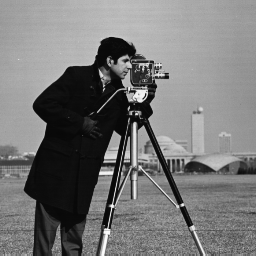
\includegraphics[width=3cm]{picture/cameraman.png}}
    \caption{cameraman}
    \label{cameraman}
\end{figure}

\begin{figure}[H]
    \centerline{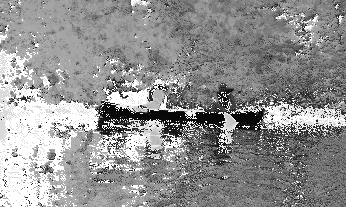
\includegraphics[width=3cm]{picture/canoe.png}}
    \caption{canoe}
    \label{canoe}
\end{figure}

\begin{figure}[H]
    \centerline{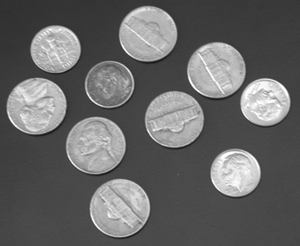
\includegraphics[width=3cm]{picture/coins.png}}
    \caption{coins}
    \label{coins}
\end{figure}

\begin{figure}[H]
    \centerline{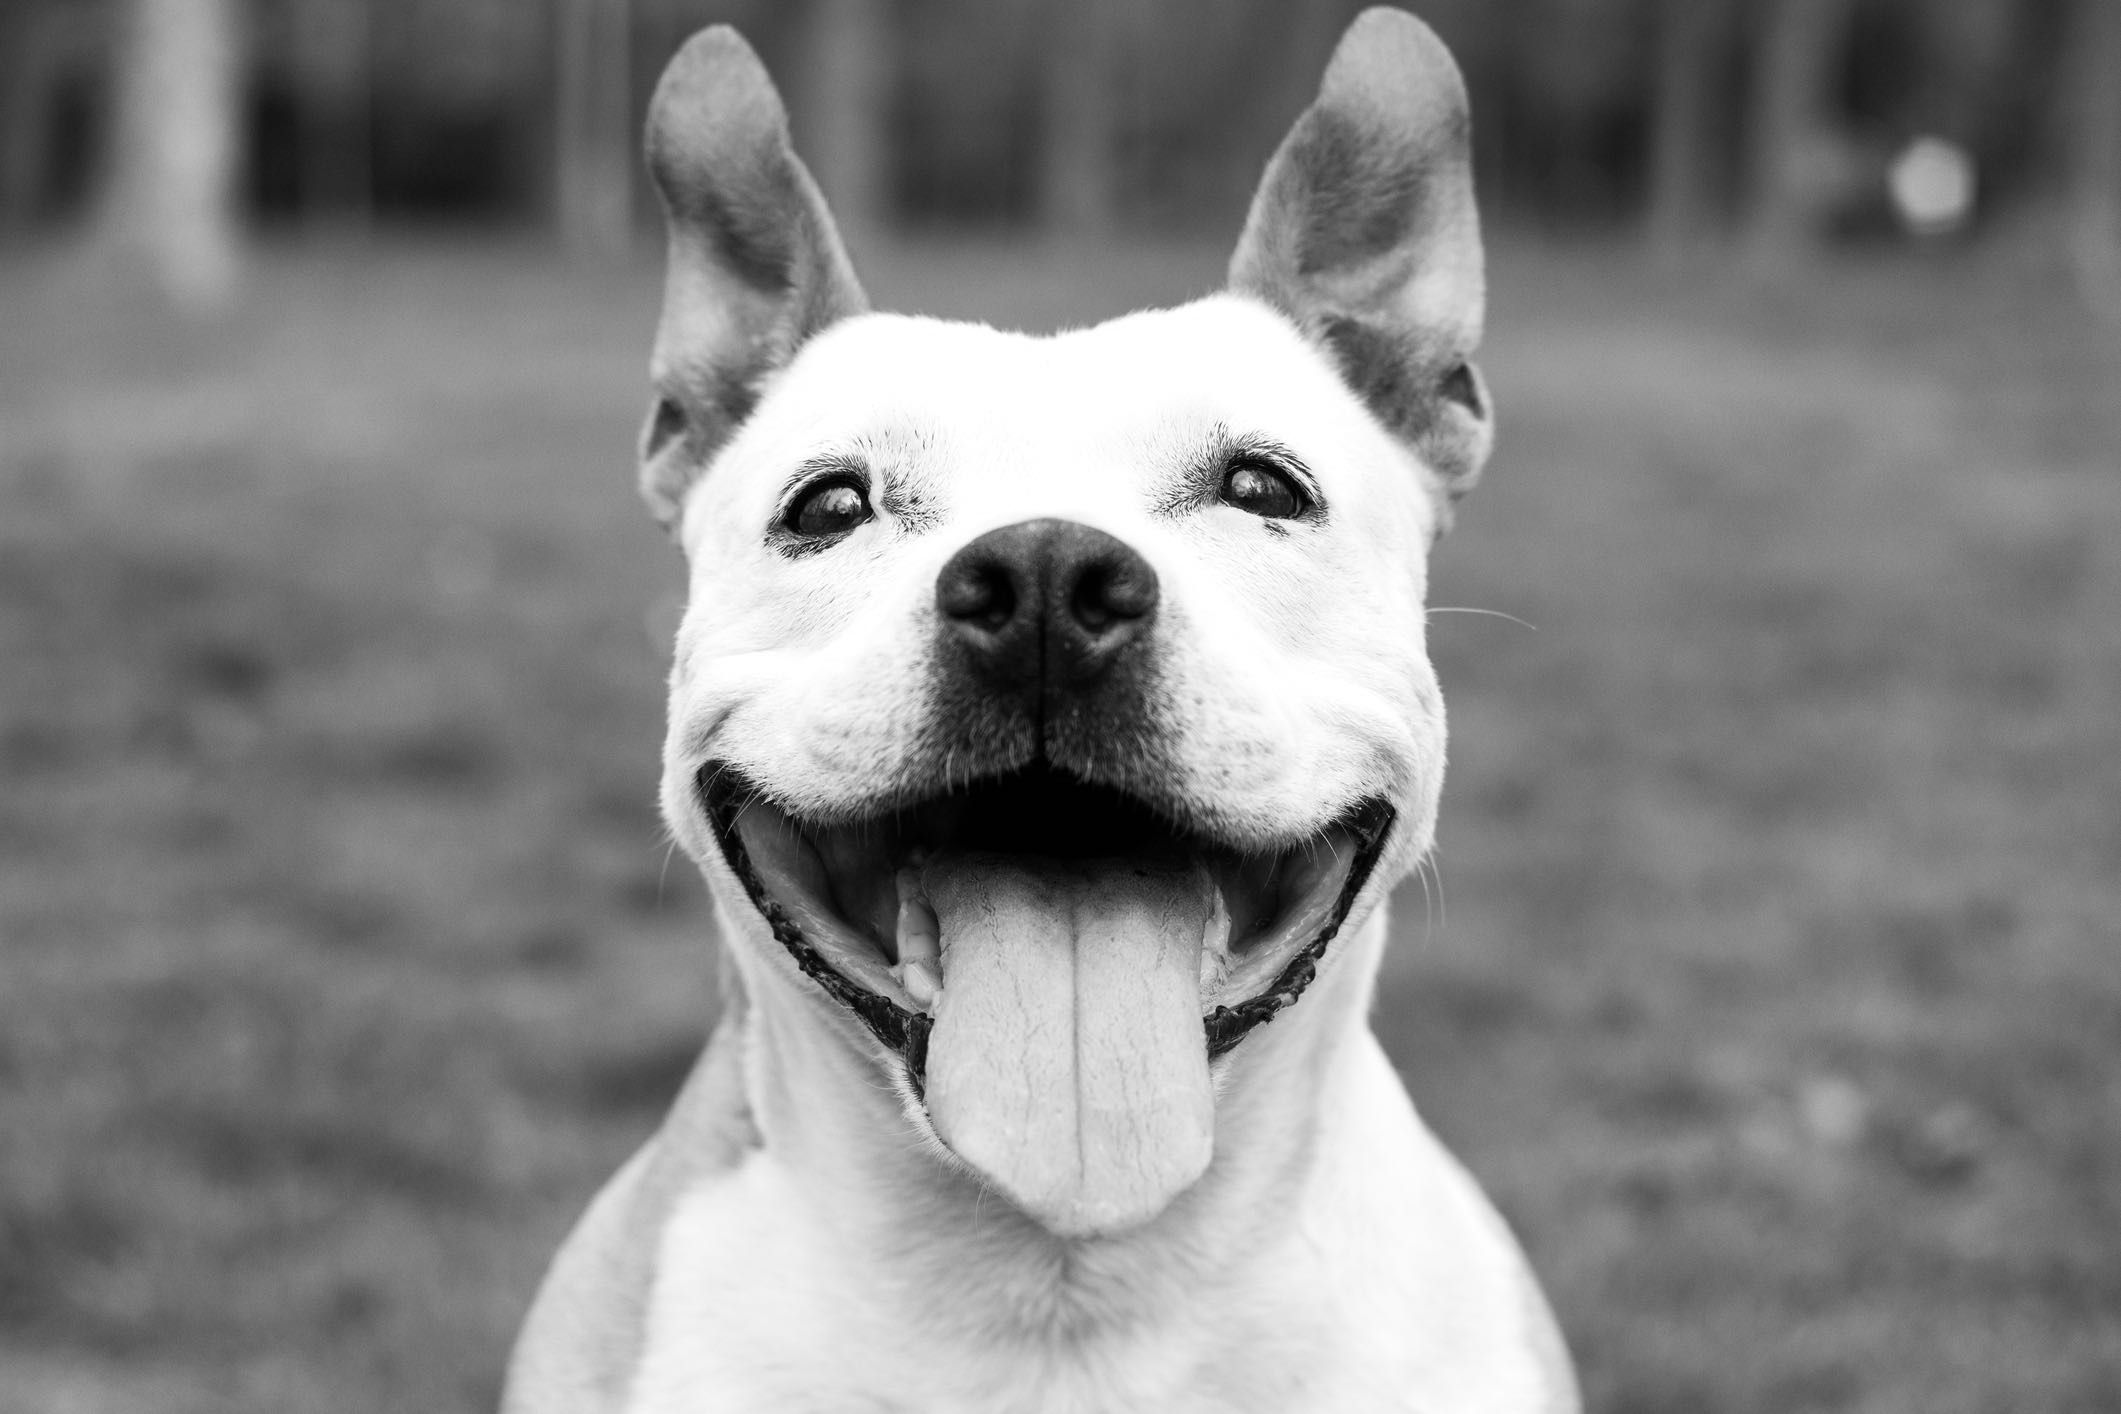
\includegraphics[width=3cm]{picture/dog.png}}
    \caption{dog}
    \label{dog}
\end{figure}

\begin{figure}[H]
    \centerline{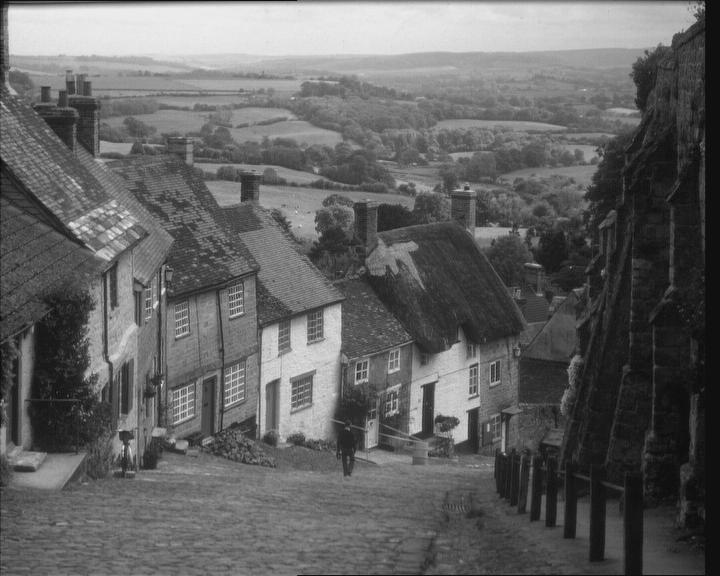
\includegraphics[width=3cm]{picture/goldhill.png}}
    \caption{goldhill}
    \label{goldhill}
\end{figure}

\begin{figure}[H]
    \centerline{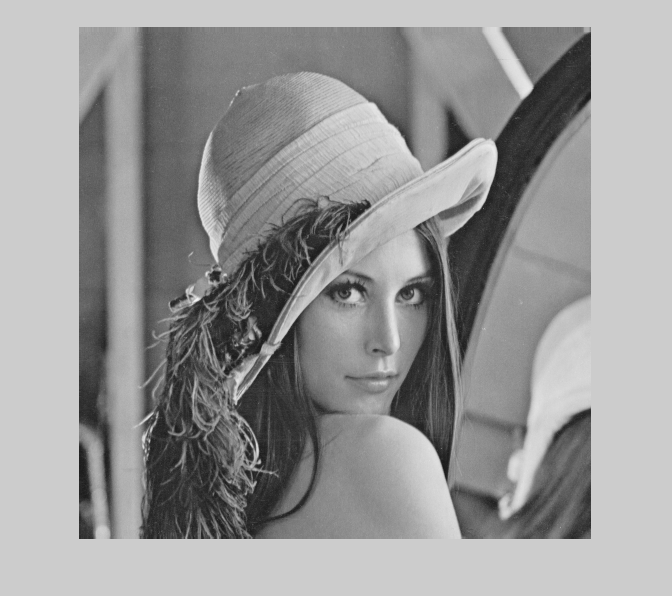
\includegraphics[width=3cm]{picture/lena.png}}
    \caption{lena}
    \label{lena}
\end{figure}

\begin{figure}[H]
    \centerline{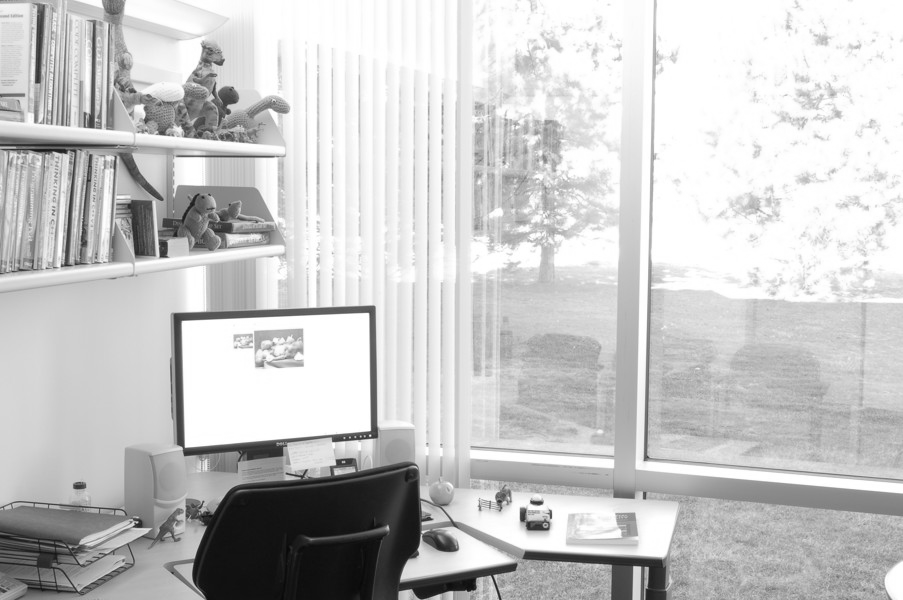
\includegraphics[width=3cm]{picture/office.png}}
    \caption{office}
    \label{office}
\end{figure}

\begin{figure}[H]
    \centerline{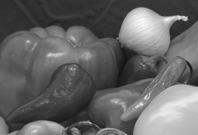
\includegraphics[width=3cm]{picture/onion.png}}
    \caption{onion}
    \label{onion}
\end{figure}

\begin{figure}[H]
    \centerline{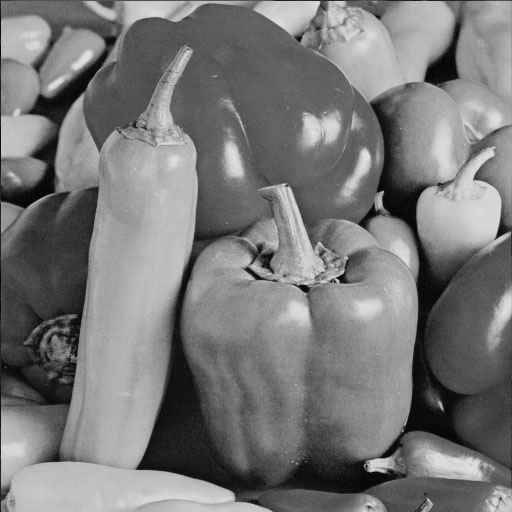
\includegraphics[width=3cm]{picture/pepper.png}}
    \caption{pepper}
    \label{pepper}
\end{figure}

Every experiment is running 30 times, we select the best result in Table I and II. We use peak signal to noise ratio (PSNR) as the performance indicator.

\begin{equation}
    \begin{aligned}
    \label{PSNR}
    PSNR=20\log_{10}(\frac{255}{RMSE}) (DB)       
\end{aligned}
\end{equation}

where RMSE is the root mean-squared error:

\begin{equation}
    \begin{aligned}
    \label{PSNR}
    RMSE=\sqrt{\frac{\sum\limits_{i=1}^{M}\sum\limits_{j=1}^{N}(I(i,j)-\hat{I}(i,j))}{M\times N}}    
\end{aligned}
\end{equation}

where $I$ is the original image, $\hat{I}$ is the image after image thresholding. Both of their size are $M\times N$.

\begin{table}[htbp]
\caption{Performance on method 1}
\begin{center}
\begin{tabular}{|c|c|c|c|c|}
    \hline
    Image & D & Fitness  & Thresholds & PSNR \\
    \hline
    bird & 2 & 5.07 & 37,56 & 38.03\\
    \hline
    & 3 & 5.07 & 16,28,55 & 36.09\\
    \hline
    & 4 & 5.07 & 40,41,41,56 & 37.08\\
    \hline
    bird2 & 2 & 5.02 & 4,6 & 27.36\\
    \hline
    & 3 & 5.02 & 0,1,5 & 27\\
    \hline
    & 4 & 4.97 & 12,16,20,23 & 27.73\\
    \hline
    cameraman & 2 & 4.86 & 5,15 & 27.95\\
    \hline
    & 3 & 4.83 & 6,14,23 & 27.91\\
    \hline
    & 4 & 4.72 & 12.,14.,39,45 & 27.91\\
    \hline
    canoe & 2 & 4.42 & 3,4 & 26.62\\
    \hline
    & 3 & 4.4 & 6,6,10 & 26.68\\
    \hline
    & 4 & 4.3 & 3,18,33,40 & 27.07\\
    \hline
    coins & 2 & 4.76 & 38,77 & 32.92\\
    \hline
    & 3 & 4.76 & 22,66,77 & 32.21\\
    \hline
    & 4 & 4.75 & 10,31,38 & 29.55\\
    \hline
    dog & 2 & 5.15 & 0,5 & 27.06\\
    \hline
    & 3 & 5.09 & 24,26,28 & 27.83\\
    \hline
    & 4 & 5.04 & 11,14,36,44 & 27.37\\
    \hline
    goldhill & 2 & 5.24 & 2,4 & 28.3\\
    \hline
    & 3 & 5.24 & 10,12,13 & 28.68\\
    \hline
    & 4 & 5.09 & 7,13,23,42 & 28.73\\
    \hline
    lena & 2 & 4 & 7,7 & 26.52\\
    \hline
    & 3 & 4 & 3,16,20 & 26.8\\
    \hline
    & 4 & 3.77 & 20,27,42 & 27.17\\
    \hline
    office & 2 & 4.93 & 2,4 & 25.21\\
    \hline
    & 3 & 4.88 & 13,15,21 & 25.46\\
    \hline
    & 4 & 4.82 & 6,36,41,42 & 25.97\\
    \hline
    onion & 2 & 5.08 & 10,10 & 28.55\\
    \hline
    & 3 & 5.07 & 5,15,25 & 28.8\\
    \hline
    & 4 & 5.06 & 2,6,9 & 28.36\\
    \hline
    pepper & 2 & 5.25 & 2,4 & 27.47\\
    \hline
    & 3 & 5.18 & 0,21,22 & 28.14\\
    \hline
    & 4 & 5.10 & 18,19,20,38 & 28.06\\
    \hline
\end{tabular}
\label{dataset_sample}
\end{center}
\end{table}

\begin{table}[htbp]
\caption{Performance on method 2}
\begin{center}
\begin{tabular}{|c|c|c|c|c|}
    \hline
    Image & D & Fitness  & Thresholds & PSNR \\
    \hline
    bird & 2 & 4.97 & 43,85 & 39.79\\
    \hline
    & 3 & 4.68 & 25,94,128 & 40.34\\
    \hline
    & 4 & 4.42 & 23,58,131,153 & 38.15\\
    \hline
    bird2 & 2 & 4.57 & 22,85 & 31.43\\
    \hline
    & 3 & 4.12 & 9,122,128 & 34.75\\
    \hline
    & 4 & 3.80 & 48,87,129,153 & 31.52\\
    \hline
    cameraman & 2 & 4.57 & 53,85 & 31.13\\
    \hline
    & 3 & 4.19 & 49,83,128 & 31\\
    \hline
    & 4 & 3.92 & 1,65,108,193 & 30\\
    \hline
    canoe & 2 & 4.12 & 71,85 & 29.93\\
    \hline
    & 3 & 3.73 & 44,87,128 & 30.05\\
    \hline
    & 4 & 3.28 & 29,83,120,153 & 29.82\\
    \hline
    coins & 2 & 4.73 & 34,85 & 33.28\\
    \hline
    & 3 & 4.55 & 57,113,128 & 34.78\\
    \hline
    & 4 & 4.34 & 20,95,103,153 & 33.76\\
    \hline
    dog & 2 & 4.81 & 73,85 & 30.92\\
    \hline
    & 3 & 4.67 & 20,77,137 & 30.39\\
    \hline
    & 4 & 4.55 & 24,66,143,153 & 29.73\\
    \hline
    goldhill & 2 & 4.81 & 23,85 & 33.39\\
    \hline
    & 3 & 4.57 & 61,97,128 & 34.42\\
    \hline
    & 4 & 4.32 & 30,72,123,153 & 32.36\\
    \hline
    lena & 2 & 3.52 & 75,85 & 29.62\\
    \hline
    & 3 & 2.85 & 36,115,128 & 31.39\\
    \hline
    & 4 & 2.12 & 13,75,129 & 29.12\\
    \hline
    office & 2 & 4.7 & 15,85 & 27.4\\
    \hline
    & 3 & 4.56 & 22,74,128 & 27\\
    \hline
    & 4 & 4.41 & 36,94,116,153 & 27.72\\
    \hline
    onion & 2 & 4.85 & 44,85 & 33.56\\
    \hline
    & 3 & 4.62 & 37,122,128 & 36.75\\
    \hline
    & 4 & 4.37 & 6,84,140,153 & 33.48\\
    \hline
    pepper & 2 & 4.82 & 64,85 & 31.68\\
    \hline
    & 3 & 4.44 & 12,66,128 & 30.4\\
    \hline
    & 4 & 4.1 & 34,65,135,153 & 30.34\\
    \hline
\end{tabular}
\label{dataset_sample}
\end{center}
\end{table}
  
\section{Conclusion}
In  this paper, we reproduce the algorithm in \cite{b1}, and revise the initializatio. Compaer two methods, method 2 is better than method 1 is PSNR. Methods 1 easliy generate solutions whose thresholds are closed. Thus, we can conclude that the proper initialization can help improve performance.

\begin{thebibliography}{00}
\bibitem{b1} Ming-Huwi Horng, Ting-Wei Jiang, Multilevel Image Thresholding Selection Based on the Firefly Algorithm, 2010 Symposia and Workshops on Ubiquitous, Autonomic and Trusted Computing
\bibitem{b2} Ping-sung Liao, Tse-sheng Chen And Pau-choo Chung, A Fast Algorithm for Multilevel Thresholding, Journal Of Information Science And Engineering 17, 713-727 (2001)
\bibitem{b3} Kapur, J.N., Sahoo, P.K., Wong, A.K.C.: A new method for gray-level picture thresholding using the entropy of the histogram, Computer Vision Graphics Image Processing, 29, 273--285, (1985).
\bibitem{b4} Yang, X.S.: Nature-inspired metaheuristic algorithms, Luniver Press,
(2008).
\end{thebibliography}
\vspace{12pt}

\end{document}
